\section{Course Introduction}


\begin{frame}
\frametitle{Course Target}
\begin{center}			

\smartdiagram[bubble diagram]{Goal,Coding,Distributed\\System,Data\\Warehouse,Big Data\\Tools,DevOps,Applications,Databases}
\end{center}
\end{frame}

%---------------------------------------------------------
%Example of the \pause command
\subsection{Learning Objectives}
\begin{frame}
\frametitle{Learning Objectives}

\begin{itemize}
    \item<1-> Understand the data management life-cycle. \pause
    \item<2-> Illustrate the basics of distributed systems concepts \pause
    \item<3-> Be familiar with ETL for (Batch/Steaming) data over distributed systems ex: Hadoop \& Spark.  \pause
    \item<4-> Apply QA and testing for the data pipeline cycle.
    \item<5-> Automate the Data life-cycle process End-to-End. \pause
    \item<6-> Building real-life examples. \pause
    \item<7-> Applying machine learning over Big Data. \pause
    \item<8-> Understanding of the DevOps tools and functions in data life-cycle. \pause
\end{itemize}

\end{frame}

%---------------------------------------------------------

\subsection{Getting max benefit from this course}

\begin{frame}
\frametitle{Getting max benefit from this course}
\begin{block}{Take the course advantage}
\begin{itemize}
	\item<1-> Follow the videos order as described. \pause
	\item<2-> Read the references for each section (including the implementation of the examples if exists). \pause
	\item<3-> Repeat the lecture code with your own.  \pause
	\item<4-> Do the assignments.\pause
	\item<5-> Ask your questions. \pause
	\item<6-> Join the online meeting or discussions. \pause
\end{itemize}
\end{block}

\end{frame}

%---------------------------------------------------------

\subsection{Assignments and Labs}
\begin{frame}
\frametitle{Assignments and Labs}
\begin{block}{Remark}
\begin{itemize}
	\item<1-> Full project code.
	\item<2-> Notebooks (Jupyter or Zeppelin).
	\item<3-> Read the reference.
\end{itemize}
\end{block}
\end{frame}

%---------------------------------------------------------

\subsection{Course Textbooks}
\begin{frame}
\frametitle{Textbooks-1}
	\begin{itemize}
		\item<1-> Hadoop: The Definitive Guide: Storage and Analysis at Internet Scale 4th Edition by Tom White.
		\item<2-> Learning Spark by Matei Zaharia, Patrick Wendell, Andy Konwinski, Holden Karau
		\item<3-> High Performance Spark Best Practices for Scaling and Optimizing Apache Spark By Holden Karau, Rachel Warren.
		\item<4-> Kafka: The Definitive Guide by Todd Palino, Gwen Shapira, Neha Narkhede.
		\item<5-> Guide to High Performance Distributed Computing: Case Studies with Hadoop, Scalding and Spark (Computer Communications and Networks) 2015th Edition			
	\end{itemize}
\end{frame}

%---------------------------------------------------------

\begin{frame}
\frametitle{Textbooks-2}
\begin{figure}[ht]
	\begin{minipage}[c][1\width]{
				0.4\textwidth}
			\centering
		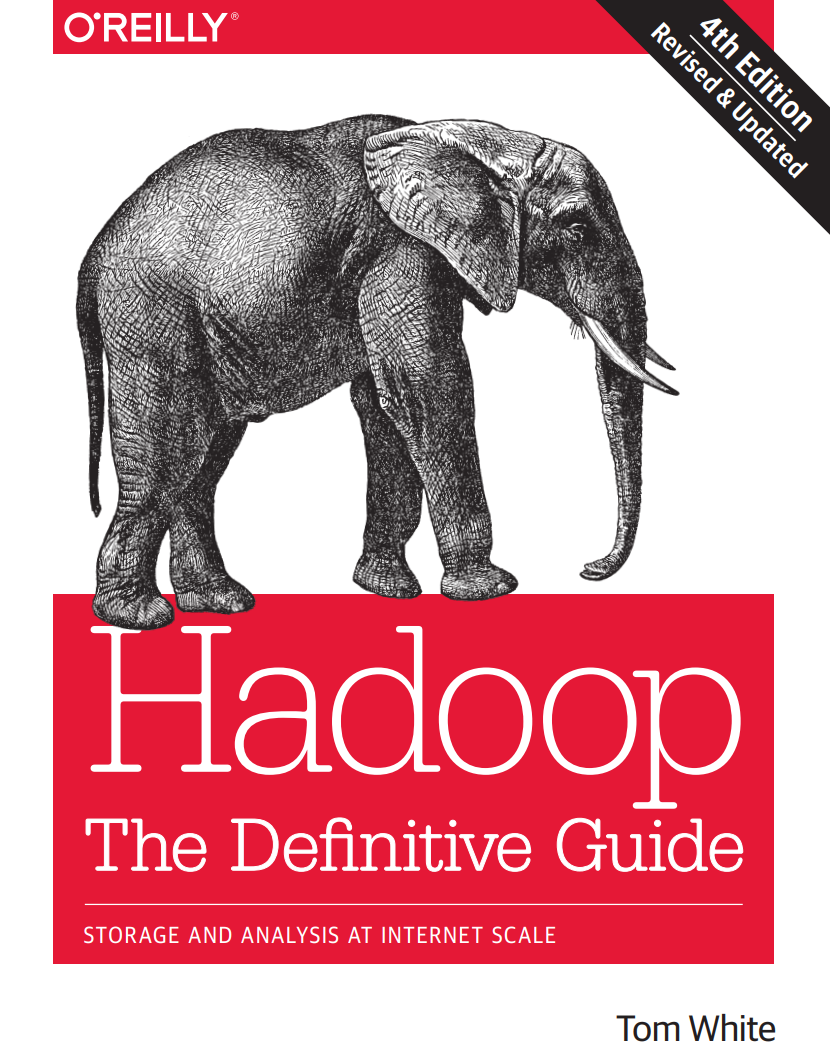
\includegraphics[width=\linewidth]{./Figures/chapter-00/hadoop-tdg.png}
	\end{minipage}
	\hfill 	
	\begin{minipage}[c][1\width]{
				0.4\textwidth}
			\centering
		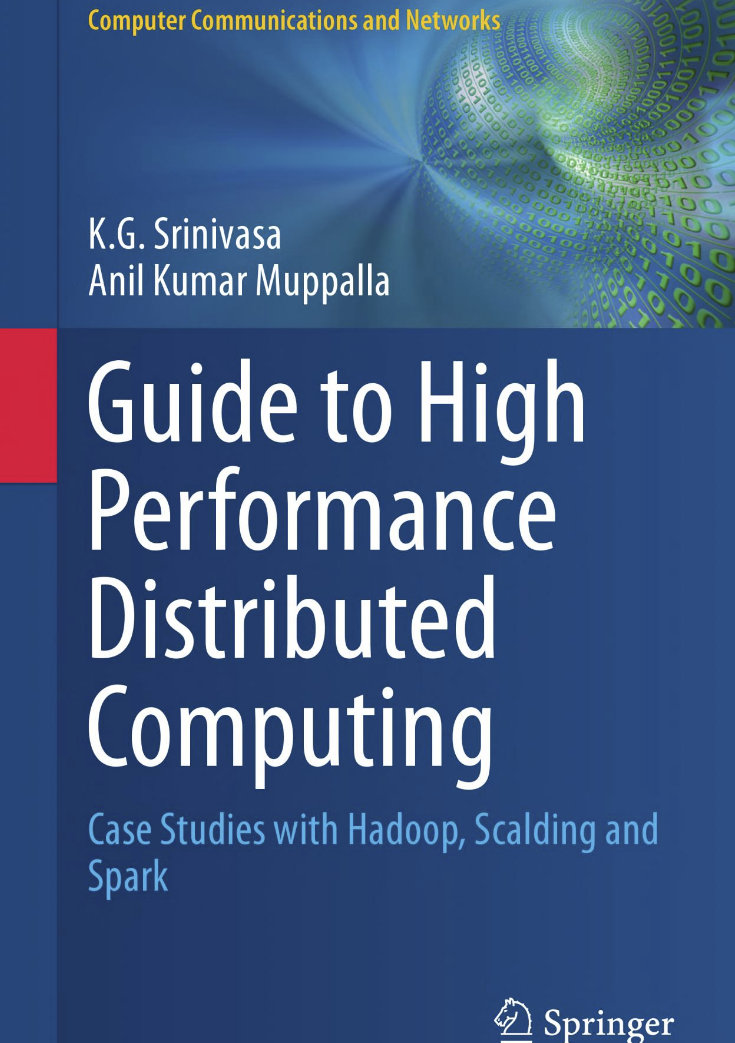
\includegraphics[width=\linewidth,height=.7\textheight]{./Figures/chapter-00/high-performance-computing.png}
	\end{minipage}
%	\caption{}
\end{figure}
\end{frame}

\begin{frame}
\frametitle{Textbooks-3}

\begin{figure}[ht]
	\begin{minipage}[c][1\width]{
			0.3\textwidth}
		\centering
		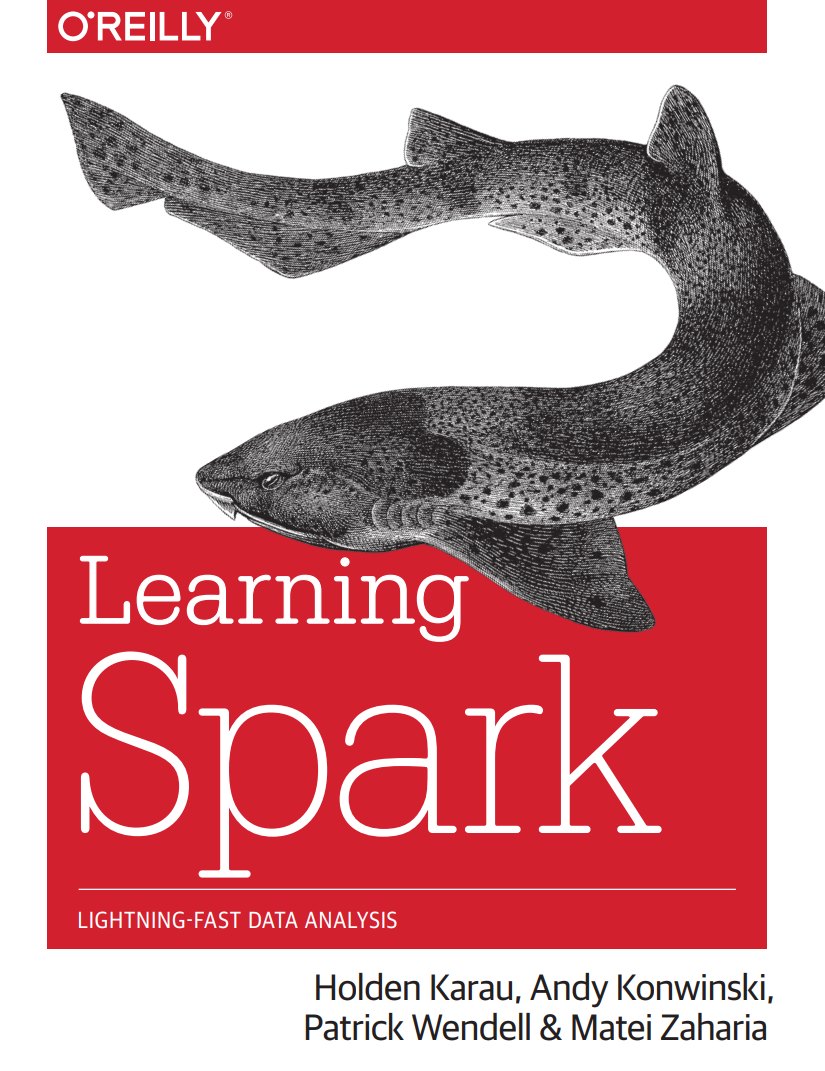
\includegraphics[width=\linewidth]{./Figures/chapter-00/learning_spark_front.png}
	\end{minipage}
	\hfill	
	\begin{minipage}[c][1\width]{
			0.3\textwidth}
		\centering
		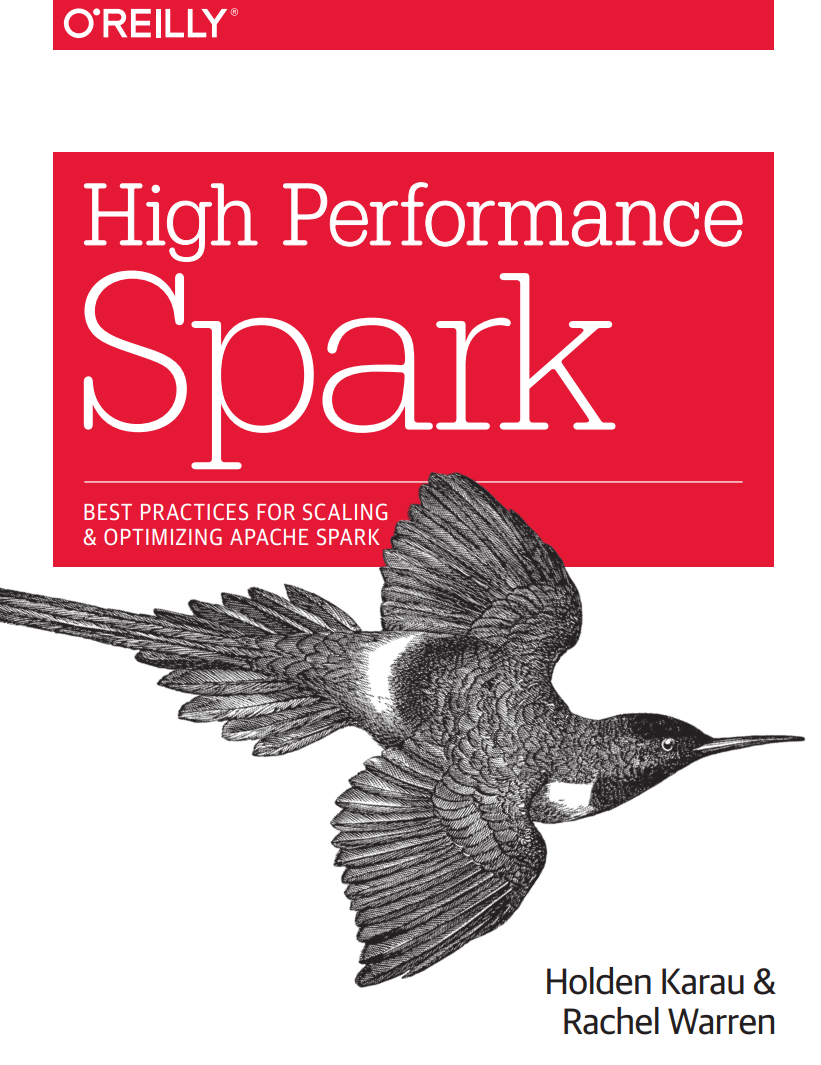
\includegraphics[width=\linewidth]{./Figures/chapter-00/spark-high-performance.png}
	\end{minipage}
\hfill
	\begin{minipage}[c][1\width]{
		0.3\textwidth}
	\centering
	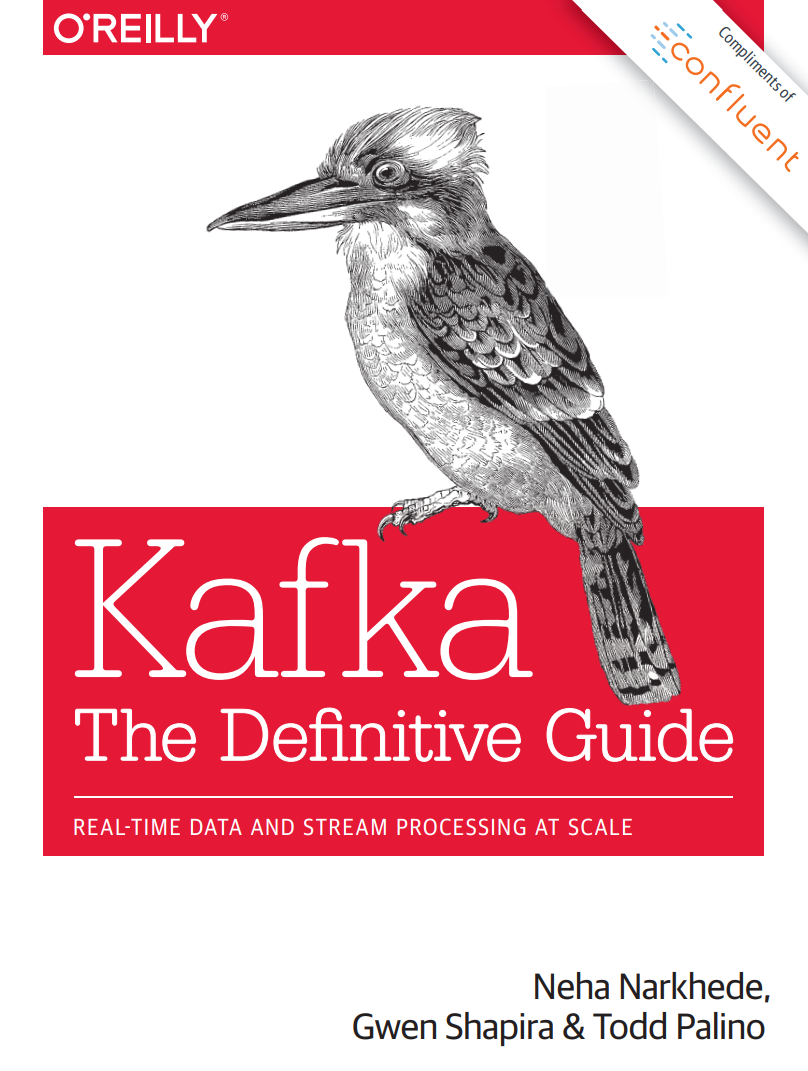
\includegraphics[width=\linewidth]{./Figures/chapter-00/kafka-tdg.png}
\end{minipage}

	%	\caption{}
\end{figure}
\end{frame}

%---------------------------------------------------------

\begin{frame}
\frametitle{Ugly but important}

\begin{itemize}
	\item User stories or technical discussions are not related to any of my current work or my previous companies.
	\item I am working at EPAM Systems. My company approved me for doing this online course public but the materials are not reviewed or assessed by my company. It is on my own responsibilities.
\end{itemize}
\end{frame}

%---------------------------------------------------------

%\begin{frame}
%\frametitle{Sample frame title}
%This is a text in second frame. For the sake of showing an example.
%
%\begin{itemize}
%    \item<1-> Text visible on slide 1
%    \item<2-> Text visible on slide 2
%    \item<3> Text visible on slides 3
%    \item<4-> Text visible on slide 4
%\end{itemize}
%\end{frame}

%%---------------------------------------------------------
%%Example of the \pause command
%\begin{frame}
%In this slide \pause
%
%the text will be partially visible \pause
%
%And finally everything will be there
%\end{frame}

%\section{Second section}
%
%%---------------------------------------------------------
%%Highlighting text
%\begin{frame}
%\frametitle{Sample frame title}
%
%In this slide, some important text will be
%\alert{highlighted} beause it's important.
%Please, don't abuse it.
%
%\begin{block}{Remark}
%Sample text
%\end{block}
%
%\begin{alertblock}{Important theorem}
%Sample text in red box
%\end{alertblock}
%
%\begin{examples}
%Sample text in green box. "Examples" is fixed as block title.
%\end{examples}
%\end{frame}
%%---------------------------------------------------------
%
%
%%---------------------------------------------------------
%%Two columns
%\begin{frame}
%\frametitle{Two-column slide}
%
%\begin{columns}
%
%\column{0.5\textwidth}
%This is a text in first column.
%$$E=mc^2$$
%\begin{itemize}
%\item First item
%\item Second item
%\end{itemize}
%
%\column{0.5\textwidth}
%This text will be in the second column
%and on a second tought this is a nice looking
%layout in some cases.
%\end{columns}
%\end{frame}
%%---------------------------------------------------------

%%%%%%%%%%%%%%%%%%%%%%%%%%%%%%%%%%%%%%%%%%%%%%%%%%%%%%%%%%%%%%%%%%%%%%%%%%%
%%% Local Variables:
%%% mode: latex
%%% TeX-master: "../main"
%%% TeX-engine: xetex
%%% End:
